\section{Architecture and Implementation}\label{sec:Architecture}
% Describe the data processing pipeline here.
% 1. Get the raw data and remove the ground (LiDAR data clean up)
% 2. Segment data and sent it to the classifier
% 3. Classification with Neural Network.

\begin{figure*}[!ht]
 \begin{center}
   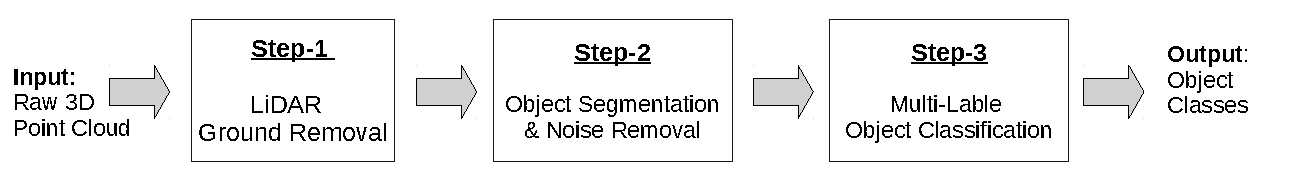
\includegraphics[width=0.85\textwidth]{./images/DataProcessingPipleline.pdf}
   \caption{Overview of our Data Processing Pipeline}
   \label{fig:dataPipeline}
 \end{center}
\end{figure*}

Our data processing pipeline consist of 3 main processing steps:

\begin{enumerate}
  \item \textbf{Step-1 Data Filtering. } Filtering the LiDAR base lines (cylinder lines around objects - See Figures \ref{fig:ground_before} and \ref{fig:after})

  \item \textbf{Step-2 Object Segmentation.} Separating the 3D point cloud to segments that contain one single object or in other words marking the object with a voxel grid.

  \item \textbf{Step-3 Object Classification.}  Classifying an object from point cloud data containing one single object.
\end{enumerate}



Figure \ref{fig:dataPipeline} depicts our data processing pipeline.
When our system runs in the testing phase, it retrieves the point cloud data for a single scene
from the DEBS2019 evaluation system which includes multiple objects and processes it in 3 steps to
deliver the classification results.

The provided training data by DEBS 2019 Challenge \cite{DEBSGC2019} includes only one single object per scene
with its label so that it is not required to have the step-2 object segmentation when we train our classifier.


% Describe \ldots.
%
% Different forms of data processing architectures that we have implemented and tested.
%
% \begin{enumerate}
%   \item Different methods for removing noise from raw data (data preprocessing).
%   \item Projecting 3D data into 2D data using 3 different projection methods
%   \item CNN  (with and without max pool) + fully-connected + dropout + fully-connected+softmax
%   \item CNN with a different number of hidden layers.
%
% \end{enumerate}
% KIA
% We need another image to describe the CNN architecture.
% Add two images about it.


\subsection{LiDAR Laser Line Data Filtering}
%KIA: Describe here how we remove the ground - keep this very general
The first step in our data processing pipeline is to filter out the LiDAR laser lines that build
a cylinder 3D shape from the laser standing point $(x=0, y=0, z=0)$. Figure \ref{fig:ground_before} visualizes the LiDAR data for a single scene with LiDAR laser lines and Figure \ref{fig:after} visualizes the data after
filtering out the Laser lines. Objects like car or pedestrian are
visible in Figure \ref{fig:after} after filtering the LiDAR lines.

This first filtering step in our data processing pipeline reduces highly the amount of data that we process and
also helps to be able to find object segments in the next following step.
We train and test the classification model (in the step-3) after removing the laser baselines and
filtering them out.
%
\begin{figure*}[!h]
\centering
\begin{minipage}{0.49\textwidth}
  \centering
        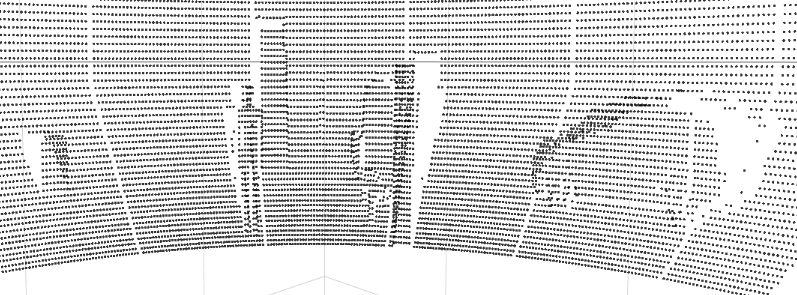
\includegraphics[width=.9\linewidth]{images/ground_before2.png}
        \caption{LiDAR Raw Point Cloud Data}
        \label{fig:ground_before}
\end{minipage}%
\begin{minipage}{0.49\textwidth}
  \centering
        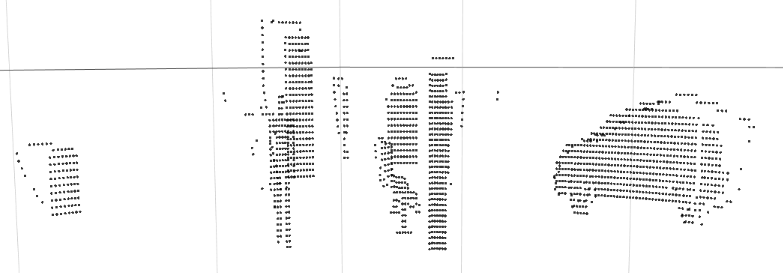
\includegraphics[width=.9\linewidth]{images/ground_after2.png}
        \caption{Data After Filtering the LiDAR Scan Lines}
        \label{fig:after}
\end{minipage}%
% \caption{General caption.} \label{fig:1}
\end{figure*}
% Describe here how we filter the ground.
%
%
\subsection{Object Segmentation and Noise Removal.}
The first step in testing phase is to segment the point cloud to chunks of data that include
possibly only one single object. For this purpose, we use different clustering
methods to cluster the data in the original 3-dimensional format and in projected 2D form.
Data points for different objects can build separate clusters.


\textbf{3D to 2D Projection.}
We have projected the 3D data in 4 different ways to a 2D plane and reduced the data dimensionality.
The first 3 data projection methods are just to consider the data by dropping one of the axes and
viewing the data from one of the sides, for examples by dropping the y-axis and considering the x
and z-axis.

The last method is to project 3D data by using a point of eye view and projecting each data points
to a plane (also named window) with a distance $d$ from eye or camera standpoint.
The following projection is used to project the point $(x,y,z)$ in 3D to new $(x',  y')$ in 2D
using a distance d to a plane.
% \large
\begin{align*}
d  & = \text{Distance to a projection plane} \\
x' & =  x (\frac{d}{z}) \ \  , \ \  y' =  y (\frac{d}{z}) \ \  , \ \  z'=  z (\frac{d}{z}) = d
\end{align*}
% \normalsize

\textbf{Object segmentation using Clustering.}
We have implemented and tested the following clustering methods to build segments of the point cloud
that contains as well as possible only one single separated object.

\begin{enumerate}
  \item \textbf{K-means and Mini Batch K-means} on the 3D and project 2D data.
  \item \textbf{Meanshift} on 3D and 2D data
  \item \textbf{DBSCAN} on 3D and 2D
\end{enumerate}

\textbf{K-means and Mini batch K-means.}
We run multiple iterations of k-means with
different batch sizes and also applied the elbow method to determine the optimal number of clusters.
Our evaluation result (Sec \ref{sec:Evaluation}) showed that the k-means algorithm cannot separate the data into one-object segments with high quality.
It also could not achieve real-time processing when we need to test the different number of clusters.

\textbf{Density based Clustering Approaches - Meanshift and DBSCAN.}
We observed that density based approaches can build better object segments in comparison to K-Means clustering mainly because of two important factors,\\
1. The density of LiDAR points is approximately equal on different objects.
In the case that there is an object, the density of points is roughly equal on the surface of
an object independent of the object type\\
2. When objects are close to each other or hiding each
other partially, density-based approaches can achieve better segments and do not joint the two different clusters of the two objects.

We have evaluated the segmentation step with different parameters (density value and number of minimum samples in each cluster).
We observed that the segments build using 3D DBSCAN approach can achieve acceptable
real-time performance and DBSCAN can build better quality segments in 3D than using the algorithm
with projected 2D data. We observed as well that the classification of object types in the
next step can fail to recognize object types correctly due to the low-quality of segment
building.


DBSCAN clustering algorithm is also used to remove the noise from the data set and return point cloud data with cluster labels.


\begin{figure*}[!h]
\begin{center}
  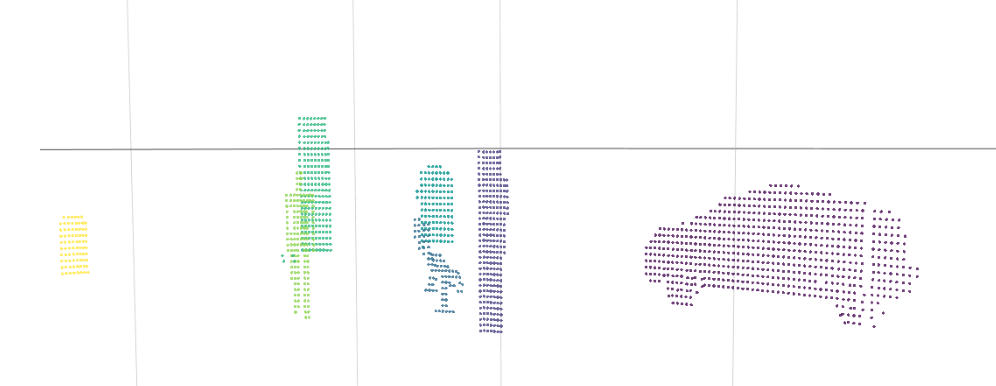
\includegraphics[width=.55\linewidth]{./images/seg_noise_removal.png}
  \caption{Clustered Point Cloud Data after Filtering the Data Noise (Colors indicate Clusters). }
  \label{fig:ClusteringWithNoiseFiltering}
\end{center}
\end{figure*}



\textbf{Sectioning From Top-View.}
To achieve better object segmentation, we developed a new approach by viewing the data from the top-view (considering data from the top elevation view (bird-view)) and projecting it to 2D. The LiDAR scanner is positioned at the center coordinate
of (0, 0, 0).  We observed that there are areas or spaces that are not occupied by any
objects and there are sections with objects inside.

Figure \ref{fig:sectors1} depicts the top-view of the LiDAR point cloud data.
The red central point is the zero point - the position of the LiDAR scanner.
All other surrounding points are object points from the top-view.

Our idea for sectioning the data from top-view is illustrated in
Figure \ref{fig:sectors2}. We calculate for each point the degree of angle that they have with the x-axis.
Angles of data points to the center will be valued between 0 and 360 degrees. We sort the list of angles
and check for ranges that we do not have data or data under certain numbers. Then we can separate the data into sectors by using the degree ranges that have no data points or less than a threshold. If the objects are very close to the LiDAR laser position, then we might have data in all ranges of angle degrees, but we would then be able
to separate the data by using a threshold value.
\begin{figure*}[!h]
\centering
\begin{minipage}{0.40\textwidth}
  \centering
         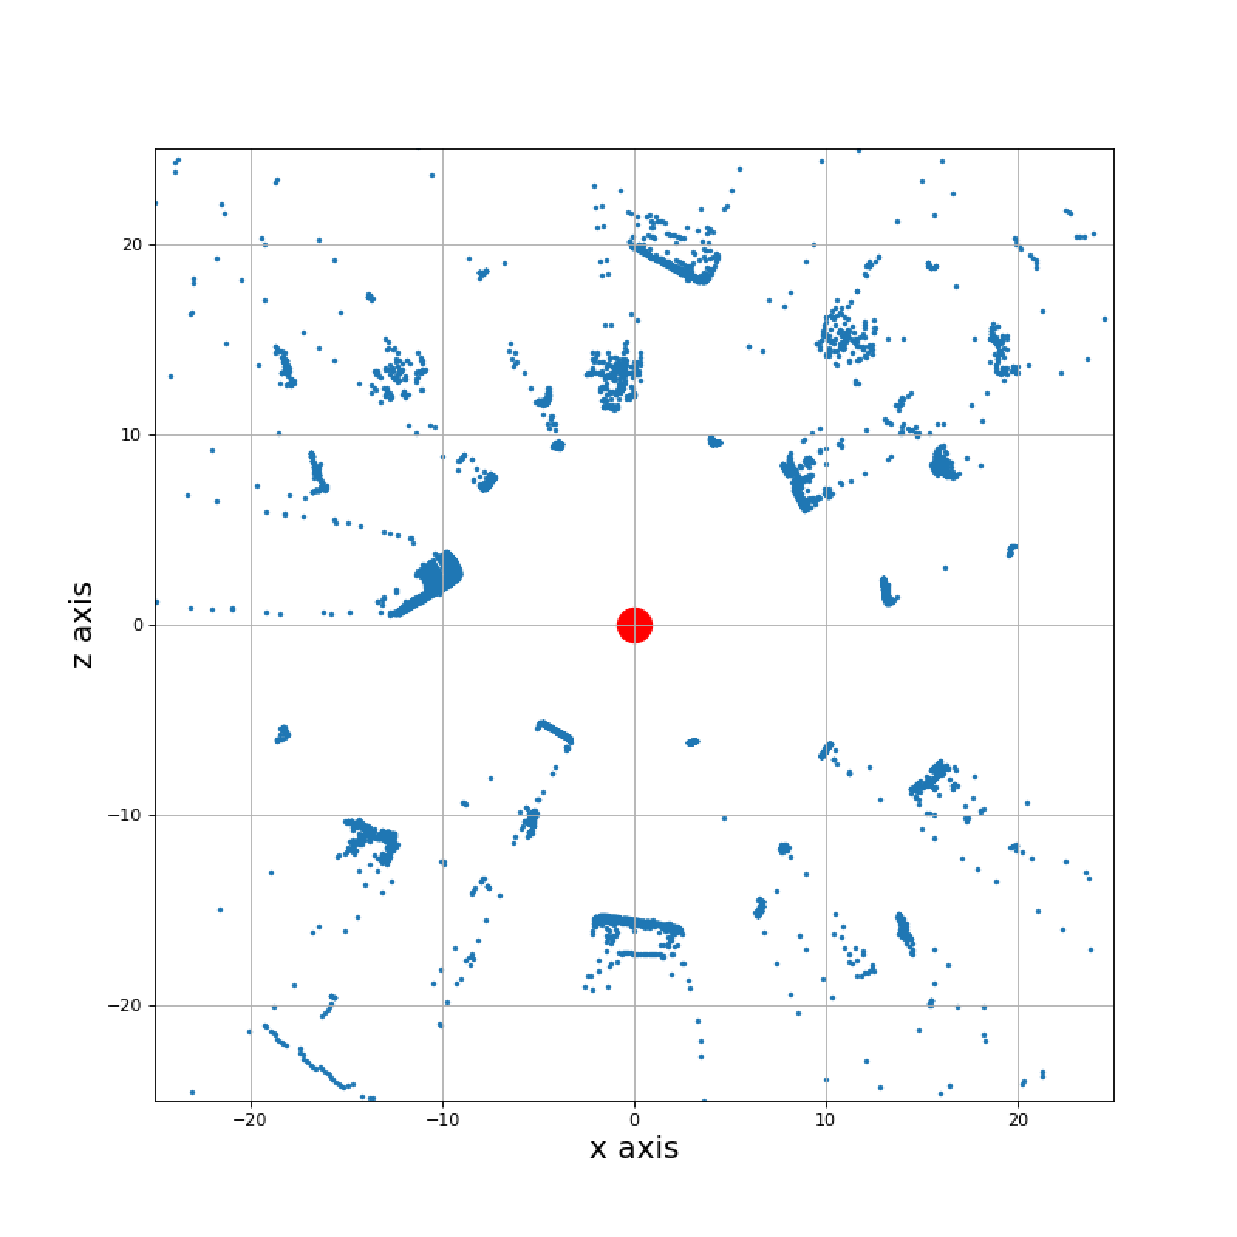
\includegraphics[scale=0.3]{./images/sector-transforms/scene-with-centre.pdf}
       \caption{Top-View of LiDAR Data}
       \label{fig:sectors1}
\end{minipage}%
\begin{minipage}{0.40\textwidth}
  \centering
        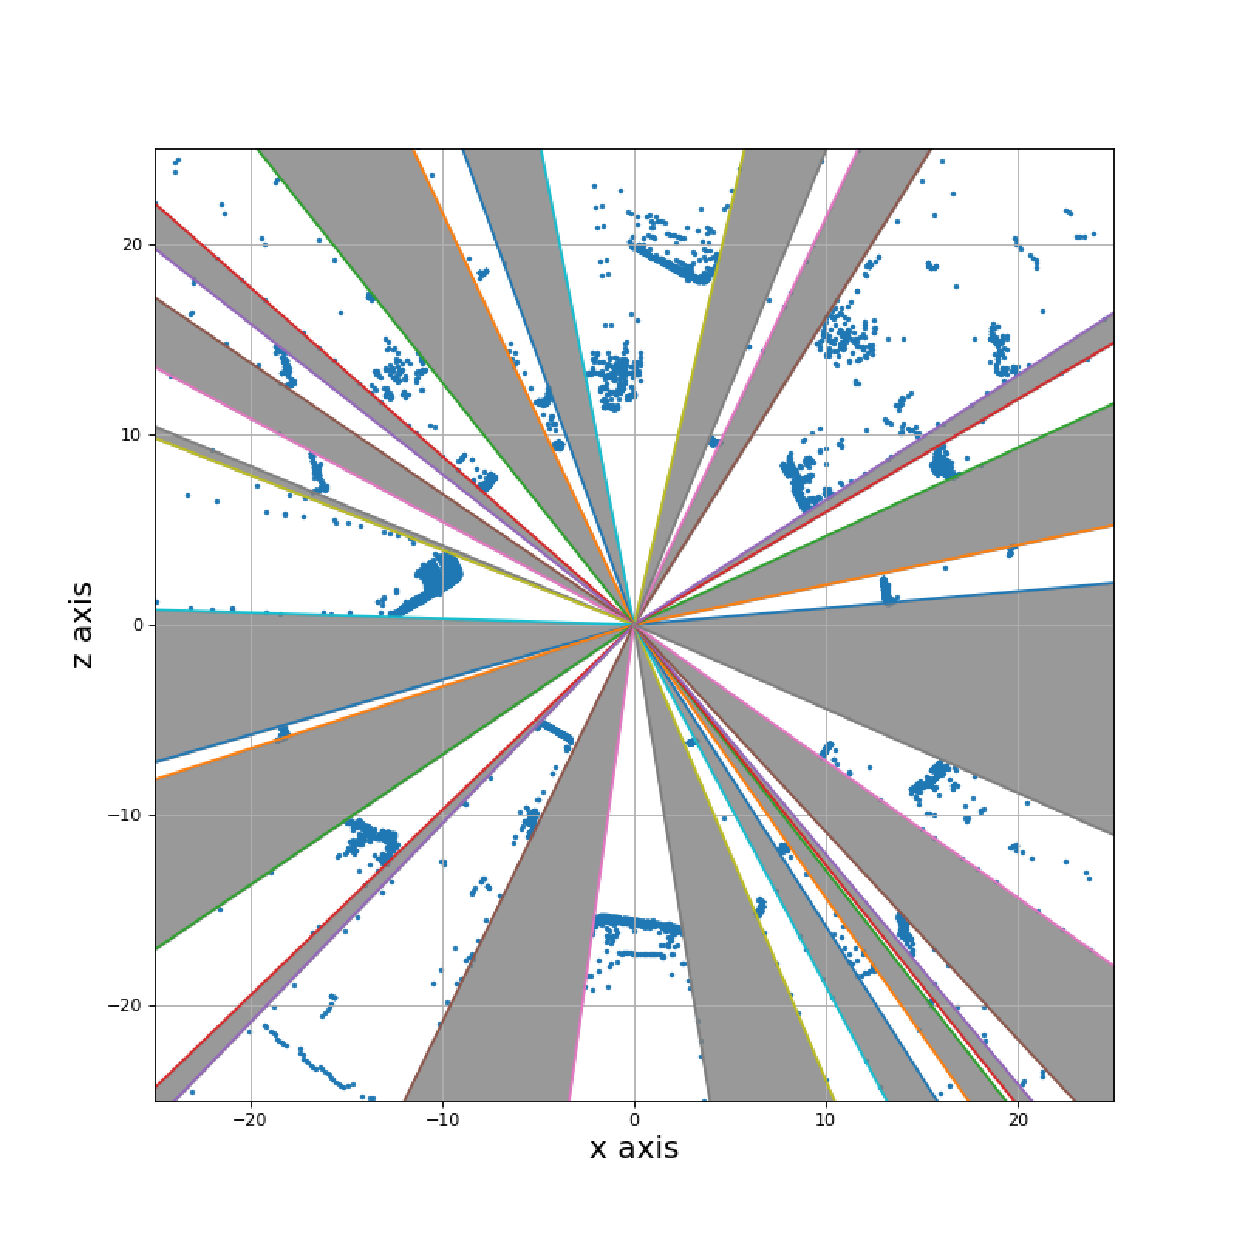
\includegraphics[scale=0.3]{./images/sector-transforms/scene-with-sector.pdf}
        \caption{Top-View - Separating unoccupied spaces/sectors (gray colored) from sectors with objects}
        \label{fig:sectors2}
\end{minipage}%
% \caption{General caption.} \label{fig:1}
\end{figure*}
The next step is to consider each sector one by one and separate data of single sector into multiple
sub-sectors if it contains multiple objects. For this purpose, we calculate the radius of each
point to the center ($\sqrt{x^2 + z^2 } $).
Then we create the density of these radius values and separate the data from the local minimums.
An example of the density curve is shown in Figure \ref{fig:SectorDensity} with 3 objects in a
sector.

It can happen that we have on a single sector objects behind each other or on each other side.
If objects are behind each other then the density value vector will have a local minimum that can
be used to separate the objects. If the density vector has local minimum points of zero then, we can separate it from the zero
points. If local minimums are very close to each other and have large values then we need to
use the density-based clustering approach like DBSCAN to build clusters.



\begin{figure}[!h]
\begin{center}
  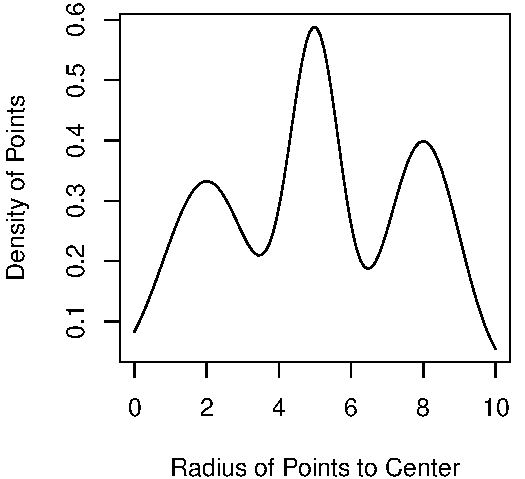
\includegraphics[scale=0.6]{./images/sectors_density.pdf}
  \caption{An Example of Density Distribution of Points in a Single Sector with 3 Objects}
  \label{fig:SectorDensity}
\end{center}
\end{figure}
Our evaluation contains segmentation with DBSCAN segmentation on 3D point cloud and on projected 2D
data without sectioning from top-view.
